\documentclass[tikz,border=6pt]{standalone}
\usepackage[T1]{fontenc}
\usepackage{lmodern}
\usepackage{amsmath,amssymb}
\usetikzlibrary{arrows.meta,calc,positioning,shapes.geometric,patterns,decorations.pathmorphing,backgrounds,fit}
\definecolor{ink}{HTML}{173948}
\definecolor{flow}{HTML}{167D9A}
\definecolor{heat}{HTML}{B75A23}
\definecolor{measure}{HTML}{70518A}
\definecolor{pale}{HTML}{EAF2F5}
\definecolor{muted}{HTML}{526571}
\definecolor{green}{HTML}{2E8665}
\tikzset{every node/.style={font=\sffamily\small,text=ink},
 equipment/.style={draw=ink,line width=1pt,fill=pale,rounded corners=2pt},
 process/.style={draw=flow,line width=1.1pt,-{Latex[length=2.4mm]}},
 signal/.style={draw=measure,dashed,line width=.9pt,-{Latex[length=2mm]}},
 thermal/.style={draw=heat,line width=1.1pt,-{Latex[length=2.3mm]}},
 labelbox/.style={fill=white,inner sep=2pt,font=\sffamily\footnotesize,align=center},
 annotation/.style={font=\sffamily\footnotesize,text=muted,align=left},
 panel/.style={draw=ink!20,fill=ink!2,rounded corners=3pt,inner sep=7pt,align=left},
 sensor/.style={circle,draw=measure,fill=white,line width=.8pt,minimum size=8mm,inner sep=1pt,font=\sffamily\scriptsize,align=center},
 box/.style={equipment,minimum width=3cm,minimum height=1.2cm,align=center}}
\newcommand{\atlasheader}[2]{\node[anchor=north west,font=\sffamily\bfseries\LARGE]at(0,0){#1};\node[anchor=north west,font=\sffamily\small,text=muted]at(0,-.75){#2};\draw[ink!25](0,-1.25)--(26,-1.25);}
\newcommand{\atlasfooter}[1]{\draw[ink!25](0,-15.8)--(26,-15.8);\node[anchor=north west,annotation,text width=25.8cm]at(0,-16){#1\\Original explanatory drawing for ThermoFuzzy-PID. Source traceability: Cordeiro (UFC, 2021), documented repository equations and explicit reconstruction choices.};}

\begin{document}
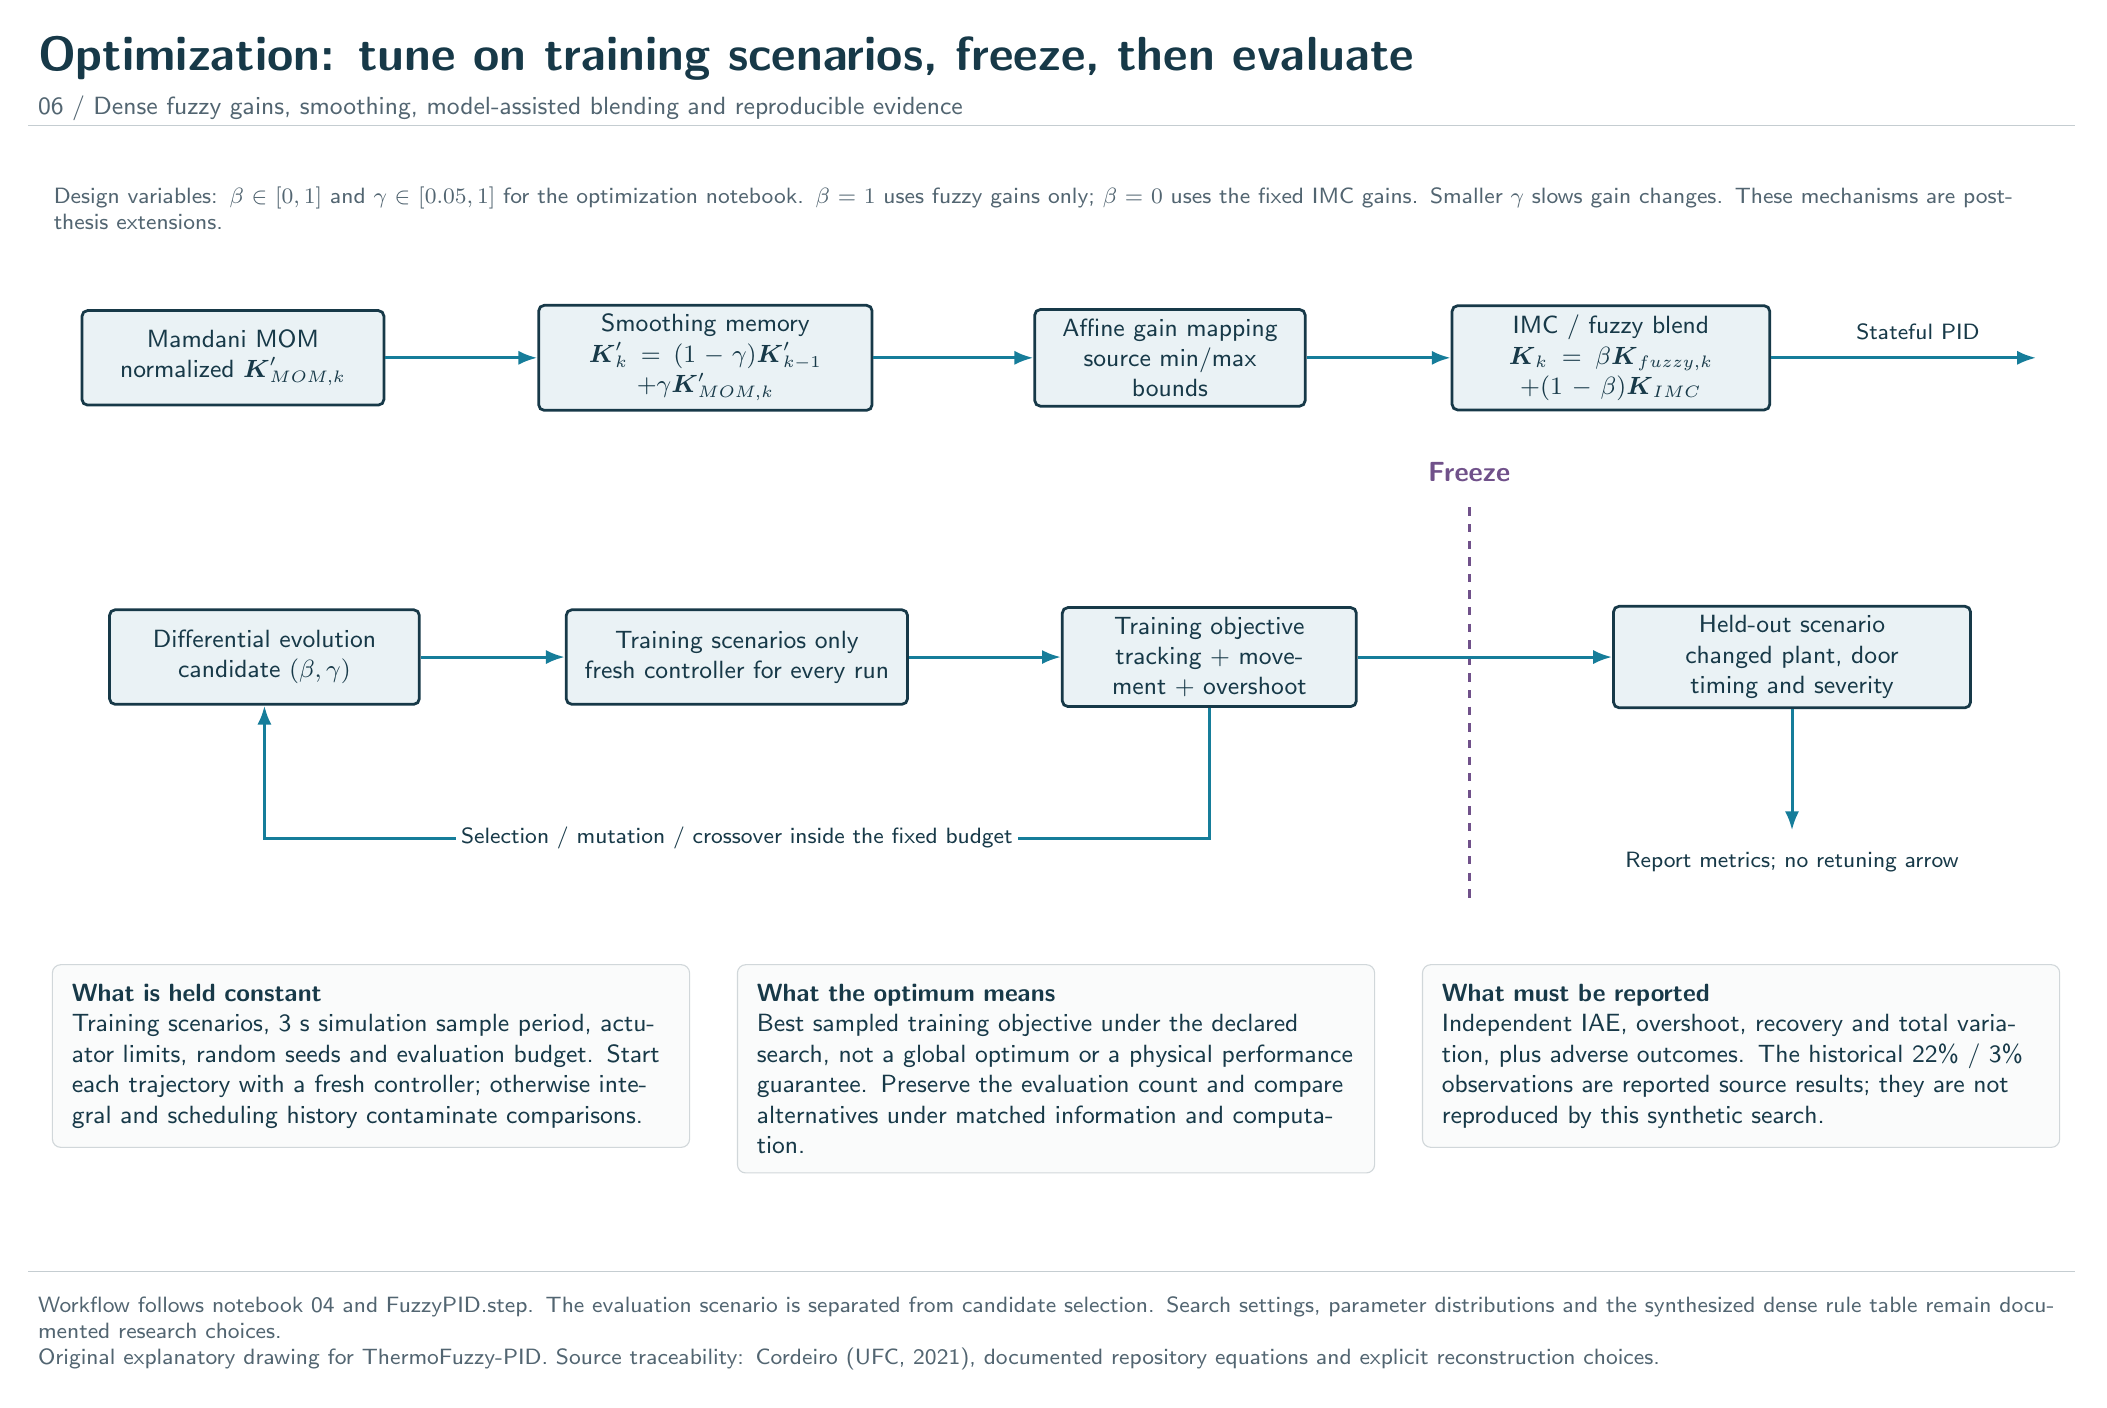
\begin{tikzpicture}[x=1cm,y=1cm]
\atlasheader{Optimization: tune on training scenarios, freeze, then evaluate}{06 / Dense fuzzy gains, smoothing, model-assisted blending and reproducible evidence}
\node[box,text width=3.6cm] (mom)at(2.6,-4.2){Mamdani MOM\\normalized $\boldsymbol K'_{MOM,k}$};
\node[box,text width=4.0cm] (smooth)at(8.6,-4.2){Smoothing memory\\$\boldsymbol K'_k=(1-\gamma)\boldsymbol K'_{k-1}$\\$+\gamma\boldsymbol K'_{MOM,k}$};
\node[box,text width=3.2cm] (scale)at(14.5,-4.2){Affine gain mapping\\source min/max bounds};
\node[box,text width=3.8cm] (blend)at(20.1,-4.2){IMC / fuzzy blend\\$\boldsymbol K_k=\beta\boldsymbol K_{fuzzy,k}$\\$+(1-\beta)\boldsymbol K_{IMC}$};
\draw[process](mom.east)--(smooth.west);
\draw[process](smooth.east)--(scale.west);
\draw[process](scale.east)--(blend.west);
\draw[process](blend.east)--(25.5,-4.2);
\node[labelbox,anchor=south]at(24.0,-4.05){Stateful PID};
\node[annotation,anchor=north west,text width=25cm]at(.2,-1.9){Design variables: $\beta\in[0,1]$ and $\gamma\in[0.05,1]$ for the optimization notebook. $\beta=1$ uses fuzzy gains only; $\beta=0$ uses the fixed IMC gains. Smaller $\gamma$ slows gain changes. These mechanisms are post-thesis extensions.};
% Optimization loop with a clear frozen test boundary.
\node[box,text width=3.7cm] (search)at(3,-8.0){Differential evolution\\candidate $(\beta,\gamma)$};
\node[box,text width=4.1cm] (train)at(9,-8.0){Training scenarios only\\fresh controller for every run};
\node[box,text width=3.5cm] (objective)at(15,-8.0){Training objective\\tracking + movement + overshoot};
\draw[process](search.east)--(train.west);
\draw[process](train.east)--(objective.west);
\draw[process](objective.south)--(15,-10.3)--(3,-10.3)--(search.south);
\node[labelbox]at(9,-10.3){Selection / mutation / crossover inside the fixed budget};
\draw[measure,dashed,line width=1.1pt](18.3,-6.1)--(18.3,-11.1);
\node[font=\sffamily\bfseries,text=measure,anchor=south]at(18.3,-5.9){Freeze};
\node[box,text width=4.3cm] (test)at(22.4,-8.0){Held-out scenario\\changed plant, door timing and severity};
\draw[process](objective.east)--(test.west);
\draw[process](test.south)--(22.4,-10.2);
\node[labelbox,anchor=north]at(22.4,-10.4){Report metrics; no retuning arrow};
\node[panel,anchor=north west,text width=7.6cm]at(.3,-11.9){\textbf{What is held constant}\\Training scenarios, 3 s simulation sample period, actuator limits, random seeds and evaluation budget. Start each trajectory with a fresh controller; otherwise integral and scheduling history contaminate comparisons.};
\node[panel,anchor=north west,text width=7.6cm]at(9.0,-11.9){\textbf{What the optimum means}\\Best sampled training objective under the declared search, not a global optimum or a physical performance guarantee. Preserve the evaluation count and compare alternatives under matched information and computation.};
\node[panel,anchor=north west,text width=7.6cm]at(17.7,-11.9){\textbf{What must be reported}\\Independent IAE, overshoot, recovery and total variation, plus adverse outcomes. The historical 22\% / 3\% observations are reported source results; they are not reproduced by this synthetic search.};
\atlasfooter{Workflow follows notebook 04 and FuzzyPID.step. The evaluation scenario is separated from candidate selection. Search settings, parameter distributions and the synthesized dense rule table remain documented research choices.}
\end{tikzpicture}
\end{document}
